\documentclass[../main/main.tex]{subfiles}
\graphicspath{{./figures/}}

\makeatletter
\renewcommand{\@chapapp}{Travaux pratiques -- TP}
\renewcommand{\chaplett}{TP}
\makeatother

% \toggletrue{student}
% \toggletrue{corrige}
% \renewcommand{\mycol}{black}
% \renewcommand{\mycol}{gray}

\hfuzz=5.003pt

\begin{document}
\setcounter{chapter}{6}

% \settype{enon}
% \settype{solu_prof}
% \settype{solu_stud}

\chapter{\cswitch{Correction du TP}{Circuits du premier ordre en r\'egime transitoire}}

\enonce{
	\begin{tcn}(appl)<ctb>"how"'t'{Capacités exigibles}
		\begin{itemize}[label=\rcheck]
			\item Distinguer, sur un relevé expérimental, régime
			      transitoire et régime permanent au cours de l'évolution d'un
			      système du premier ordre soumis à un échelon de tension.
			\item Réaliser l'acquisition d'un régime transitoire pour un circuit
			      linéaire du premier ordre et analyser ses caractéristiques.
			      Confronter les résultats expérimentaux aux expressions théoriques.
			\item Capacité numérique~: mettre en œuvre la méthode
			      d'\textsc{Euler} à l'aide d'un langage de programmation pour
			      simuler la réponse d'un système linéaire du premier ordre à une
			      excitation de forme quelconque.
		\end{itemize}
	\end{tcn}
	\vspace{-10pt}
	\section{Objectifs}
	\begin{itemize}
		\item Réaliser des montages simples d'électricité.
		\item Déterminer expérimentalement un temps de relaxation.
		\item Observer les différents paramètres qui influent sur un régime
		      transitoire.
		\item Observer les différents régimes du second ordre.
		\item Découvrir quelques fonctions nouvelles de l'oscilloscope et du GBF.
		\item Mettre en œuvre la méthode d'\textsc{Euler} à l'aide de Python pour
		      simuler la réponse d'un système linéaire du premier ordre à une
		      excitation
		      quelconque.
	\end{itemize}

	\section{S'approprier}

	\begin{tcb}(rapp){Règles de bonne pratique}
		\begin{itemize}
			\item En pratique, on commence toujours par effectuer les branchements du
			      circuit sans insérer les appareils de mesure.
			\item Puis, on \textbf{relie toutes les masses entre elles} afin d'éviter
			      de fixer par erreur une autre masse dans le circuit. Ainsi, un bon
			      circuit aura une «~ligne de masse~» à laquelle seront reliés
			      obligatoirement tous les câbles noirs provenant des câbles
			      coaxiaux-filaires reliés à l'oscilloscope ou au GBF.
			\item Enfin, on place alors les fils colorés des câbles de mesure aux
			      endroits où on désire relever la tension. Vous serez d'ailleurs
			      également vigilant-es au choix de couleurs des fils, sinon on se perd
			      rapidement…
		\end{itemize}
		Ces règles sont fondamentales et ne doivent pas être négligées si
		on veut que le circuit fonctionne.
	\end{tcb}

	\subsection{Circuit intégrateur}

	Un montage est considéré comme \textbf{intégrateur} (on le verra en cours dans
	quelques semaines) si la tension de sortie (dans notre cas $u_{c}(t)$) est une
	primitive, à une constante multiplicative $K$ près, de la tension d'entrée
	(dans notre cas $e(t)$), soit encore

	\[u_{c}(t) = K \int e(t) \dt\]

	\subsection{Détermination numérique de la solution}
	\subsubsection{Position du problème}

	Soit $u_{C}(t)$ est solution de l'équation différentielle~:
	\[
		\dv{u_C(t)}{t} + \frac{u_C(t)}{\tau} = \frac{e(t)}{\tau}
	\]

	L'objectif de cette partie est de déterminer \textbf{numériquement} la
	solution $u_{C}(t)$ de cette équation pour une entrée quelconque $e(t)$ pour
	laquelle il n'existe pas toujours de solutions analytiques. Nous allons
	utiliser un schéma numérique classique appelé Méthode d'\textsc{Euler}.

	En pratique, cette méthode est relativement peu efficace (et des méthodes plus
	sophistiquées sont souvent mises en place). Néanmoins la méthode
	d'\textsc{Euler}, très simple à comprendre et à mettre en place, permet une
	première approche simple du problème.

	\subsubsection{Méthode d'\textsc{Euler}~: mathématiquement}
	\label{sssec:euler}

	Des théorèmes assurent que, sous des conditions raisonnables, il existe une
	unique application $y$ de classe $C^1$ sur $[a,b]$ dont la valeur est imposée
	en $a$ et qui vérifie une équation différentielle de la forme
	$y'(t)=f(t,y(t))$ pour tout $t \in [a,b]$. L'objet des \textit{schémas
		numériques} est d'obtenir des approximations de cette solution.
	\bigbreak
	\noindent
	\begin{minipage}[c]{.55\linewidth}
		En pratique, on tente d'approcher $y$ en un certain nombre de points
		répartis sur l'intervalle $[a,b]$. Plus précisément, on veut calculer une
		approximation $y_k$ des $y(t_k)$ avec $t_k=a+kh$ où $h=\dfrac{b-a}{n}$ est
		un pas qu'il conviendra d'ajuster (on peut supposer que plus le pas est
		petit, meilleure sera l'approximation). De façon simple, on peut écrire~:
		\begin{align*}
			y(t_{k+1})-y(t_k) & =
			\int_{t_k}^{t_{k+1}}y'(u) \dd u =
			\int_{t_k}^{t_{k+1}} f(u,y(u)) \dd u
			\\\Lra
			y(t_{k+1})-y(t_k) & \approx h f(t_k,y(t_k))
		\end{align*}
	\end{minipage}
	\hfill
	\begin{minipage}[c]{.45\linewidth}
		~
		\begin{center}
			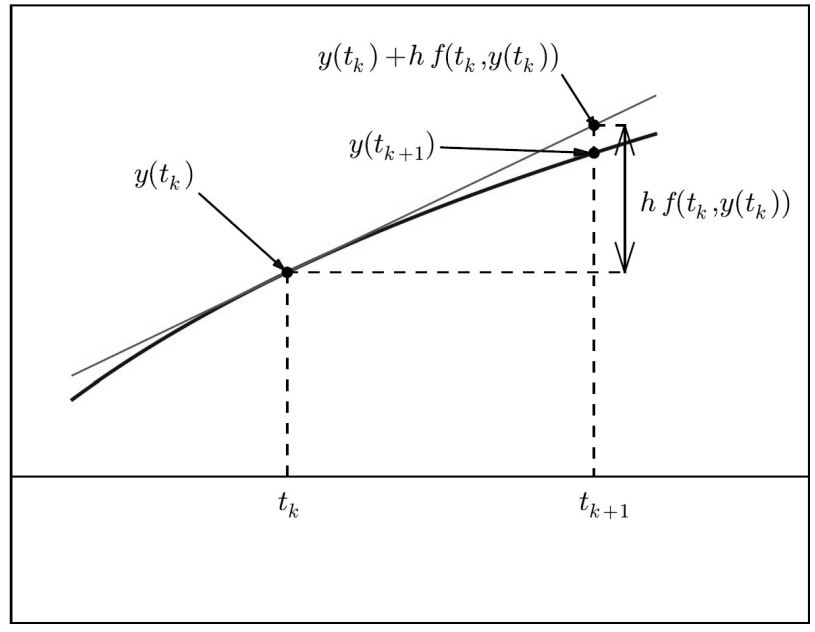
\includegraphics[width=\linewidth]{euler}
		\end{center}
	\end{minipage}
	\bigbreak
	On obtient alors la méthode d'\textsc{Euler} explicite~: les approximations
	sont calculées de proche en proche via la formule suivante~:
	\[\boxed{y_{k+1}=y_k+hf(t_k,y_k)}\]
	On initialise bien entendu avec $y_0=y(a)$, qui sera la seule valeur
	«~exacte~» calculée.
}

\setcounter{section}{2}
\section{Analyser~: régime transitoire du circuit RC}

\enonce{
	\begin{tcb}[cnt, bld](impo){}
		Vous prendrez soin de refaire tous les schémas des circuits mis en place ou
		étudiés.
	\end{tcb}
}

\subsection{Charge et décharge du condensateur}
\label{ssec:chdech}
\setlist[blocQR,1]{leftmargin=10pt, label=\clenumi}

On considère le montage ci-contre de constante de temps $\tau = RC$.

\noindent
\QR[2]{%
	\begin{minipage}[t]{.65\linewidth}
		Si $e(t)$ est une tension créneau de fréquence $f = \SI{1}{kHz}$,
		quelle valeur faut-il donner à $\tau$ pour visualiser de façon
		satisfaisante la totalité du régime transitoire~? Expliquer les raisons
		de votre choix.
	\end{minipage}
	\hfill
	\begin{minipage}[t]{.35\linewidth}
		~
		\vspace{-50pt}
		\begin{center}
			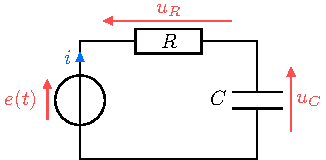
\includegraphics[width=\linewidth]{circ_rc-start}
		\end{center}
	\end{minipage}
}{%
	\noindent
	\begin{minipage}[t]{.65\linewidth}
		La tension créneau de fréquence $f$ a pour période $T = 1/f$. Pour
		visualiser correctement le signal, il faut que le condensateur puisse se
		charger sur \textbf{une demi-période} $T/2$. Or, un condensateur met
		$\approx 5\tau$ à se charger~; il nous faut donc
		\begin{gather*}
			5\tau \leq \frac{T}{2}
			\Lra
			5\tau \leq \frac{1}{2f}
			\Lra
			\boxed{\tau \leq \frac{1}{10f}}
			\qav
			\left\{
			\begin{array}{rcl}
				f & = & \SI{1e3}{Hz}
			\end{array}
			\right.\\
			\AN
			\xul{
				\tau \leq \SI{1e-4}{s} = \SI{0.1}{ms}
			}
		\end{gather*}
	\end{minipage}
	\hfill
	\begin{minipage}[t]{.35\linewidth}
		~
		\begin{center}
			\includegraphics[width=\linewidth]{creneau_taugood}
			\captionof{figure}{}
		\end{center}
	\end{minipage}
}

\QR<[start=2]>[1]{%
	Si $\tau$ est trop grand ou si $\tau$ est trop petit, que se
	passe-t-il~?
}{%
	\begin{itemize}
		\item Si $\tau$ est \textbf{trop grand}, le condensateur n'aura \textbf{pas
			      le temps de se charger}. On ne verra qu'une portion de
		      l'exponentielle croissante.
		\item À l'inverse, si $\tau$ est \textbf{trop petit}, le condensateur se
		      \textbf{charge trop vite}~: on confondra la courbe de sa charge avec
		      celle du créneau.
	\end{itemize}
}

\QR[1]{%
	Si $R = \SI{1}{k\Omega}$, quelle valeur faut-il alors donner à $C$~?
}{%
	Prenons $\tau = \SI{1e-4}{s}$. On a~:
	\begin{gather*}
		\tau = RC
		\Lra
		\boxed{C = \frac{\tau}{R}}
		\qav
		\left\{
		\begin{array}{rcl}
			\tau & = & \SI{1e-4}{s}
			\\
			R    & = & \SI{1}{k\ohm}
		\end{array}
		\right.\\
		\AN
		\xul{
			C = \SI{1e-7}{F} = \SI{0.1}{\micro F}
		}
	\end{gather*}
}

\QR[1]{%
	On veut visualiser à l'oscilloscope simultanément $e(t)$ sur la voie 1
	et $u_{C}(t)$ sur la voie 2~; indiquer sur un schéma les connexions à
	réaliser.
}{%
	\begin{center}
		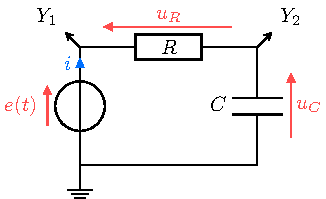
\includegraphics[scale=1]{circ_rc-start_q4-voies}
		\captionof{figure}{}
	\end{center}
}

\subsection{Étude théorique du circuit intégrateur}
\label{ssec:cint}

\enonce{%
	L'équation différentielle vérifiée par $u_{C}(t)$ est
	\[
		\dv{u_{C}(t)}{t} + \frac{u_{C}(t)}{\tau} = \frac{e(t)}{\tau}
	\]
	Supposons que à $t=0$, $e(t)$ passe de $0$ à $E$.
}

\QR[2]{\label{q:sol}%
	Déterminer la solution de l'équation différentielle précédente dans
	le cas où $u_{C}(t=0) = 0$. En utilisant un développement limité du
	terme exponentiel autour de $t = 0$, montrer que le montage est
	intégrateur (la sortie est une primitive de l'entrée).
	\begin{tcn}[aide](expe)<itc>""{Aide}
		Le développement limité de l'exponentiel s'écrit
		\[\exr^{x} \Sim_{x \to 0} 1+x\]
	\end{tcn}
}{%
	L'équation homogène est~:
	\begin{DispWithArrows*}[]
		\dv{u_{C,h}}{t} + \frac{1}{\tau}u_{C,h} &= 0
		\Arrow{Forme générale homogène}
		\\\Ra
		u_{C,h}(t) &= A\exp\left( -\frac{t}{\tau} \right)
		\Arrow{$u_{C,p}(t) = \lambda$}
		\\\Ra
		0 + \frac{\lambda}{\tau} &= \frac{E}{\tau}
		\Arrow{$\lambda = E$}
		\\\Lra
		u_{C,p}(t) &= E
		\Arrow{$u_{C}(t) = u_{C,h}(t) + u_{C,p}(t)$}
		\\\Ra
		u_C(t) &= E + A\exp \left( - \frac{t}{\tau} \right)
		\Arrow{Par continuité}
		\\\Ra
		u_{C}(0) &= 0 = E+A
		\\\Lra
		A &= -E
		\Arrow{On combine}
		\\\Ra
		\Aboxed{u_C(t) &= E\left(1-\exp\left(-\frac{t}{\tau}\right)\right)}
	\end{DispWithArrows*}
	Quand $\frac{t}{\tau} \ra 0$, on utilise le développement limité~:
	\begin{gather*}
		u_{C}(t) \Sim_{t/\tau \to 0}
		E \left( 1 - \left( 1 - \frac{t}{\tau} \right) \right)
		\\\Ra
		\boxed{u_C(t) \Sim_{t/\tau \to 0} \frac{Et}{\tau}}
	\end{gather*}
	Or, une primitive de $\int E \dd{t}$ est $Et$~: on obtient bien que dans ce
	cas, le montage est intégrateur (à $\tau$ près).
}

\subsection{Circuit RC avec visualisation de $e(t)$ et $u_{R}(t)$}
\label{ssec:uR}

\enonce{%
	On souhaite maintenant visualiser $e(t)$ sur la voie 1 et $u_{R}(t)$ sur la
	voie 2.
}


\QR[1]{%
	Comment faut-il modifier le montage~? Sur votre feuille, faire le
	schéma du montage correspondant en indiquant les branchements de
	l'oscilloscope.
}{%
	\begin{center}
		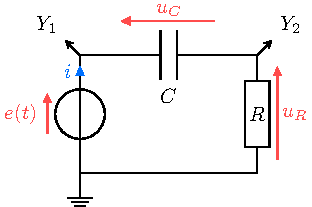
\includegraphics[scale=1]{circ_rc-start_q6-voies}
		\captionof{figure}{}
	\end{center}
}

\QR[2]{%
	Écrire l'équation différentielle vérifiée par la variable $u_{R}(t)$
	et en donner la solution pour $e(t) = E$ et $u_{R}(t=0^-) = 0$.
	Attention, la tension n'est \textit{a priori} pas continue aux bornes de
	$R$…
}{%
	Pour obtenir l'équation sur $u_R$ ou $i(t)$, il suffit de \textbf{dériver la
		loi des mailles}~:
	\begin{DispWithArrows*}[]
		u_R + u_C &= E
		\CArrow{$\dv{t}\/(~)$}
		\\\Ra
		\dv{u_R}{t} + \dv{u_C}{t} &= 0
		\Arrow{$\dv{u_C}{t} = \frac{i}{C}$ et $i = \frac{u_R}{R}$}
		\\\Lra
		\dv{u_R}{t} + \frac{u_R}{RC} &= 0
		\Arrow{$\tau = RC$}
		\\\Lra
		\Aboxed{\dv{u_R}{t} + \frac{u_R}{\tau} &= 0}
	\end{DispWithArrows*}
	On résout mais en faisant attention à la condition initiale. Pour cela, on
	étudie la loi des mailles en $t = 0^{+}$~:
	\begin{DispWithArrows*}
		u_R(0^{+}) + u_C(0^{+}) &= E
		\Arrow{$u_C(0^{+}) = 0$ par continuité}
		\\\Ra
		\Aboxed{u_R(0^{+}) &= E}
	\end{DispWithArrows*}
	L'ED étant déjà homogène, on aura $u_R(t) = A'\exr^{-\frac{t}{\tau}}$, et avec
	la condition initiale précédemment trouvée on a directement
	\[
		\boxed{u_R(t) = E\exr^{-\frac{t}{\tau}}}
	\]
	On peut vérifier la cohérence de cette solution en la réinjectant dans la loi
	des mailles~:
	\begin{gather*}
		u_R + u_C = \cancel{E\exr^{-\frac{t}{\tau}}} +
		E \left( 1 - \cancel{\exr^{-\frac{t}{\tau}}} \right)
		\\\Lra
		\boxed{u_R + u_C = E}
	\end{gather*}
	ce qui est bien la réponse attendue.
}

\section{Réaliser et valider}
\subsection{Étude expérimentale du régime transitoire du circuit RC}

\subsubsection{Cas général~: charge et décharge du condensateur}

\setlist[blocQR,1]{leftmargin=10pt, label=\sqenumi}
\resetQ
\enonce{%
	\begin{tcb}(expe){}
		\begin{enumerate}
			\item Réaliser le montage RC proposé dans la partie~III.A.
			\item $e(t)$ est une tension créneau (alternance de tension nulle et de
			      tension constante $E$) d'un générateur basses fréquences, réglé sur
			      une fréquence de $\SI{1}{kHz}$.
			\item $R$ est une boîte de résistances variables~; prendre $R =
				      \SI{1}{k\Omega}$.
			\item $C$ est une boîte de capacités réglables~; prendre la valeur calculée
			      dans la partir analyse.
			\item Observer $e(t)$ et $u_{C}(t)$.
			\item Imprimer vos courbes en suivant le protocole imprimé et plastifié sur
			      vos paillasses. \textbf{Pensez à inverser la couleur de l'écran pour
				      le pas imprimer sur un fond noir}.
		\end{enumerate}
	\end{tcb}
}

\QR[0.5]{%
	Déterminer la constante de temps $\tau_{\exp}$ ainsi que son
	incertitude. Expliquer votre démarche.
}{%
	Sur les courbes imprimées, on trouve $\tau_{\exp}$ avec soit la méthode de la
	tangente, soit à l'intersection avec $\num{0.632}E$ pour le RC en charge ou
	$\num{0.368}E$ pour le RC en décharge.
}

\QR[0.5]{%
	Calculer \textbf{et commenter} l'écart normalisé $E_N$ avec la valeur
	théorique.
}{%
	On estime l'incertitude sur $\tau_{\exp}$ \textit{via} l'incertitude de
	lecture avec la règle, par exemple. La valeur théorique comprend les
	incertitudes sur $R$ et $C$ (à vérifier sur les composants en TP). On calcule
	\[
		E_N =
		\frac{\abs{\tau_{\exp} - \tau_{\rm theo}}}
		{\sqrt{u(\tau_{\exp})^{2} + u(\tau_{\rm theo})^{2}}}
	\]
	et la mesure est cohérente et validée si $E_N \lesssim 2$.
}

\QR[0.5]{%
	Étudier l'influence de $R$ et de $C$. Faire varier également la
	fréquence du signal périodique. Commenter vos observations. Il n'est pas
	demandé de refaire de nouvelles mesures. Une analyse qualitative est
	suffisante.
}{%
	$R$ et $C$ on la même influence sur le temps de charge, puisque $\tau = RC$~:
	augmenter l'une des deux caractéristiques augmente le temps de charge, coupant
	la courbe observée~; à l'inverse, baisser l'une des deux réduit le temps de
	charge et fait se confondre $u_C$ avec $e(t)$.
	\smallbreak
	La fréquence va également influencer le signal. En effet, pour que le circuit
	ait le temps de charger, il faut que la (demi)-période soit suffisamment
	grande ($T/2 > 5\tau$). Évidemment, augmenter la fréquence diminue la période
	et on observe plus de créneaux si on ne change pas le calibre horizontal, mais
	ce qu'il faut observer (après recalibrage) c'est qu'\textbf{augmenter la
		fréquence empêche la charge totale du RC}. Ça revient à augmenter le temps de
	charge. Diminuer la fréquence a l'effet inverse.
}

\subsubsection{Cas particulier du circuit intégrateur}

\enonce{%
	\begin{tcb}*[cnt, bld](impo)"bomb"{Attention}
		Pour toute mesure, vérifier que la source du menu mesure correspond bien à
		la courbe sur laquelle vous faites des mesures.
	\end{tcb}
}

\begin{enumerate}
	\item Ne pas modifier le montage précédent, $e(t)$ est toujours une tension
	      créneau. Choisir $\tau$ de l'ordre de $5T$ en ajustant la valeur de
	      $R$ et observer $e(t)$ et $u_{C}(t)$.
	      \QR[0.5]{%
		      Quelle est l'allure de $u_{C}(t)$~? $u_{C}(t)$ est-elle bien la
		      primitive de $e(t)$ à une constante multiplicative près?
	      }{%
		      Avec $\tau$ «~trop grand~», le signal de sortie est très faible. En
		      effet, on se trouve alors dans la situation du développement limité de
		      la question~\ref{q:sol}, soit
		      \[
			      u_C(t) \Sim_{\frac{t}{\tau} \to 0} \frac{Et}{\tau}
		      \]
		      En diminuant le calibre vertical, on observe cependant le signal~: il
		      s'assimile à des portions de droites, croissantes quand $e(t) = E$ et
		      décroissantes quand $e(t) = 0$~: c'est bien une primitive de la
		      fonction, mais divisée par $\tau$.
	      }
	      \QR[0.5]{%
		      Déterminer expérimentalement la pente de la courbe $u_{C}(t)$ en
		      vous aidant des curseurs. Comparer à la valeur théorique.
	      }{%
		      On doit trouver une pente de $\frac{E}{\tau}$.
	      }
	\item Conserver les valeurs de $\tau$ et $T$. Changer la tension créneau par
	      une tension sinusoïdale.
	      \QR[0.5]{%
		      Quelle est l'allure de $u_{C}(t)$~? Le circuit est-il toujours
		      intégrateur~?
	      }{%
		      $u_C(t)$ ressemble à une fonction sinusoïdale. Le circuit reste
		      intégrateur, puisqu'on observe une différence de phase d'environ
		      $\pi/2$ par rapport à l'entrée $e(t)$.
	      }
	      \QR[0.5]{%
		      Quelle est l'expression mathématique (aucun calcul à effectuer)
		      de la courbe $u_{C}(t)$~?
	      }{%
		      \[
			      \boxed{u_C(t) = K\sin(2\pi ft) = K\sin(2\pi \frac{t}{T})}
		      \]
		      puisque $u_C(0) = 0$.
	      }
	\item Conserver les valeurs de $\tau$ et $T$. Changer la tension créneau par
	      une dent de scie.
	      \QR[0.5]{%
		      Quelle est l'allure de $u_{C}(t)$~? Le circuit est-il à priori
		      toujours intégrateur~?
	      }{%
		      L'intégrale d'une fonction affine est un polynôme du second degré. Si
		      $u_C(t)$ est une primitive de $e(t)$, on doit donc observer des
		      portions de paraboles de forme
		      \[
			      u_C(t) \propto t^{2}
		      \]
		      mais toujours continue (puisque $u_C(t)$ est continue).
		      \smallbreak
		      Bien qu'elle ressemble à une courbe sinusoïdale, on observe une
		      différence lors du changement de régime qui nous indique qu'on obtient
		      bien des paraboles~: \fbox{le circuit est toujours intérateur}.
	      }
	      \QR[0.5]{%
		      Quelle est l'expression mathématique (aucun calcul à effectuer)
		      de la courbe $u_{C}(t)$~?
	      }{%
		      On s'attend à avoir
		      \[
			      \boxed{u_C(t) = at^{2}}
		      \]
		      pour vérifier $u_C(0) = 0$. On pourait penser avoir un terme linéaire
		      en temps, mais le signal d'entrée semble linéaire et pas affine.
	      }
	      \def\lspace{30}
	\item Augmenter $\tau$.
	      \QR[0.5]{%
		      Quel inconvénient apparaît~? Commenter vos observations.
	      }{%
		      Si on augmente \textbf{encore} $\tau$, le signal $u_C(t)$ devient trop
		      faible. Le bruit du circuit domine sur la tension, et il devient
		      difficile de bien distinguer sa forme.
	      }
\end{enumerate}

\def\lspace{30}

\subsubsection{Tension aux bornes de la résistance $u_R$}

Se placer dans les mêmes conditions que dans la partie III.C, en revenant à une
tension créneau pour $e(t)$. Observer à l'oscilloscope $e(t)$ et $u_{R}(t)$.
\QR<[start=11]>[1]{%
	Imprimer les résultats. Commenter l'allure
	de la courbe. Est-elle conforme à l'expression analytique attendue~?
}{%
	On observe une \textbf{discontinuité de la tension} $u_R(t) = Ri(t)$ à chaque
	changement de la tension d'entrée, avec une croissance ou décroissance
	exponentiele. Cela correspond bien à l'expression analytique attendue, et au
	fait que l'intensité dans un circuit $RC$ n'est \textbf{pas continue}.
}

\subsection{Étude numérique}
% \begin{myverbbox}{\pya}
% def euler(f, a, b, y0, n):
%   h = (b-a) / n
%   list_y = [y0]
%   yk = y0
%   tk = a
%   for k in range(n):
%   yk = # à compléter
%   tk = # à compléter
%   list_y.append(yk)
%   return list_y
% \end{myverbbox}
% \begin{myverbbox}{\pyb}
% list_y = euler(f, 0 , 10, 0, n) # list_y est un vecteur des valeurs de y
% \end{myverbbox}
\enonce{%
Effectuez cette étude sur \texttt{Capytale}~:
\url{https://capytale2.ac-paris.fr/web/c/bc8f-2174341}.

\subsubsection{Écriture du script}

% Vous avez dans un premier temps besoin d'importer les bibliothèques Python
% suivantes~:
%
% \begin{python}
% import matplotlib.pyplot as plt
% import numpy as np
% \end{python}

On créé la fonction \texttt{euler(f, a, b, y0, n)} effectuant les calculs
détaillés dans la partie~\ref{sssec:euler}. Ses paramètres d'entrée sont
une fonction $f$, des valeurs de $a$ et $b$, un entier $n$ et une
condition initiale $y0$. Elle calcule les valeurs approchées sur $[a,b]$ de la
solution de l'équation différentielle $y'(t)=f(t,y(t))$ avec la condition
initiale $y(a)=y0$. Cette fonction renvoie la liste des $n+1$ valeurs
approchées $y_k$ de $y$ aux temps $t_k=a+k \frac{b-a}{n}$, $k\in[\![0,n]\!]$.

% Compléter ensuite la fonction \texttt{euler(f, a, b, y0, n)} suivante qui, étant
% donnée une fonction $f$, des valeurs de $a$ et $b$, un entier $n$ et une
% condition initiale $y0$, calcule les valeurs approchées sur $[a,b]$ de la
% solution de l'équation différentielle $y'(t)=f(t,y(t))$ avec la condition
% initiale $y(a)=y0$. Cette fonction renverra la liste des $n+1$ valeurs
% approchées $y_k$ de $y$ aux temps $t_k=a+k \frac{b-a}{n}$, $k\in[\![0,n]\!]$.

% \pya

\begin{tcb}(code)<lfnt>{Code}
	\vspace{-10pt}
	\inputpygments[numbers=left,xleftmargin=10pt]{python}{python/TP07_euler.py}
\end{tcb}

Il faut ensuite créer la fonction \texttt{f} ainsi que la fonction entrée
\texttt{e} pour plus de clarté. Vous compléterez la fonction \texttt{f} pour
qu'elle renvoie l'expression correspondant à l'équation différentielle que
vous cherchez à résoudre.

% \begin{python}
% def f(t, y, e):
%   return # à compléter
%
% def e(t):
%   return 10 # à modifier, par exemple np.sin(t)
% \end{python}
%
% L'exemple proposé ici est dans le cas d'une entrée constante d'amplitude $E =
%   10$. Vous pouvez alors changer la fonction \texttt{e(t)} si vous voulez explorer
% les solutions pour d'autres formes d'entrée.

On récupére les valeurs $y$ de la solution par~:
% \pyb
% tau = 1 # s
% list_t = np.linspace(0, 10, n+1) # vecteur temps entre t = 0 et t = 10 s
\begin{tcb}(code)<lfnt>{Code}
	\vspace{-10pt}
	\inputpygments[numbers=left,xleftmargin=10pt]{python}{python/TP07_val-y.py}
\end{tcb}
}%

\setcounter{subsubsection}{1}
\subsubsection{Test dans un cas analytique}
\enonce{%
	Tester votre fonction précédente avec une entrée constante $e(t) = E$ afin de
	résoudre l'équation différentielle sur $u_{C}(t)$. Afficher sur un même
	graphique la solution numérique et la solution analytique obtenue
	question~\ref{q:sol} (avant développement limité). On pourra, par choix et pour
	fixer les idées, sans que cela porte à conséquence prendre~:

	\[
		E = \SI{1}{V}
		\qquad \qquad
		\tau = \SI{1}{s}
		\qquad \qquad
		u_{C}(t=0) = 0
	\]

	Vous afficherez également la fonction erreur au cours du temps, qui est la
	différence entre votre solution numérique et la solution analytique.
}

\QR[5]{%
	Quelle est la sensibilité au pas de calcul~? Vous ferez plusieurs essais.
}{%
	Plus le pas est petit ($n$ grand), plus la détermination est fidèle. Avec trop
	peu de points, l'approximation par une tangente est mauvaise, et on s'écarte
	du résultat.
}

\ifcorrige{L'activité corrigée est disponible à
	\url{https://capytale2.ac-paris.fr/web/c/64ab-2283618}}

\enonce{%
	\subsubsection{Test dans un cas non analytique}

	Lorsque la solution $u_{C}(t)$ peut être obtenue analytiquement, la solution
	numérique n'a que peu d'intérêt. Elle prend en revanche tout son sens dans des
	cas non-analytiques.
	\smallbreak
	Testez votre programme pour plusieurs entrées (en changeant le contenu de la
	fonction \texttt{e(t)})~: sinusoïdale, rampe linéaire, exponentielle…
}

\end{document}
